\documentclass[12pt]{article}

\usepackage[T1,T2A]{fontenc}
\usepackage[utf8]{inputenc}
\usepackage[bulgarian]{babel}
\usepackage{graphicx}
\usepackage{amssymb}
\usepackage{amsmath}
\usepackage{commath}
\usepackage{float}
\usepackage{booktabs}   
\usepackage{ltablex}

\parindent 0px % turn off indenting

% have nicer-looking links
\usepackage{hyperref}
\hypersetup{
  colorlinks   = true, %Colours links instead of ugly boxes
  urlcolor     = red, %Colour for external hyperlinks
  linkcolor    = blue, %Colour of internal links
  citecolor   = blue
}
\usepackage[hypcap=true]{caption}


%%%%%%%%%%%%%%%%%%%%%%%%%%%%%%%%%%%%%%%%%%%%%%%%%%
%%%%%%%%%%%%%%%% START OF PREAMBLE %%%%%%%%%%%%%%%
%%%%%%%%%%%%%%%%%%%%%%%%%%%%%%%%%%%%%%%%%%%%%%%%%%

\newcommand{\JMUTitle}[9]{

  \thispagestyle{empty}
  \vspace*{\stretch{1}}
  {\parindent0cm
  \rule{\linewidth}{.7ex}}
  \begin{flushright}
    \vspace*{\stretch{1}}
    \sffamily\bfseries\Huge
    #1\\
    \vspace*{\stretch{1}}
    \sffamily\bfseries\large
    #2\\
    \vspace*{\stretch{1}}
    \sffamily\bfseries\small
    #3
  \end{flushright}
  \rule{\linewidth}{.7ex}

  \vspace*{\stretch{1}}
  \begin{center}
    
\includegraphics[width=3in]{./images/logo.png} \\
    \vspace*{\stretch{1}}
    \Large Курсов проект по \\ \textit{Извличане на информация} \\

    \vspace*{\stretch{2}}
    \large Факултет по математика и информатика\\
    \large Софийски университет\\
    
    \vspace*{\stretch{1}}
    \large Лектор: #8 \\[1mm]
    
    \vspace*{\stretch{1}}
    \large #7 \\

  \end{center}
}

\newcommand*{\MyIndent}{\hspace*{7em}}

%%%%%%%%%%%%%%%%%%%%%%%%%%%%%%%%%%%%%%%%%%%%%%%%%%
%%%%%%%%%%%%%%%%% END OF PREAMBLE %%%%%%%%%%%%%%%%
%%%%%%%%%%%%%%%%%%%%%%%%%%%%%%%%%%%%%%%%%%%%%%%%%%


\begin{document}  

  \JMUTitle
      {Ati: Система за разпознаване на авторство}
      {Симеон Христов}
      {6MI3400191}
      
      {Wirtschaftswissenschaftlichen Fakultät}  % Name der Fakultaet
      {W"urzburg 2018}                          % Ort und Jahr der Erstellung
      {Февруари 2023}                              % Tag der Abgabe
      {проф. Иван Койчев}               % Name des Erstgutachters
      {Zweitgutachter}                          % Name des Zweitgutachters

  \clearpage

\tableofcontents

\clearpage



%%%%%%%%%%%%%%%%%%%%%%%%%%%%%%%%%%%%%%%%%%%%%%%%%%
% УВОД
%%%%%%%%%%%%%%%%%%%%%%%%%%%%%%%%%%%%%%%%%%%%%%%%%%

\section{Увод}

Целта на проекта е създаването на система за категоризация, която при даден корпус от документи - $D$, всеки от които е написан от един автор $y$, идентифицира автора на анонимен текст $x$.

\vspace{1em}

Разработената система може да бъде основата за разработване на приложение, което да:

\begin{enumerate}
    \item \textbf{Проверява на авторство}: Дали даден текст наистина е написан от определен автор?
    \item \textbf{Открива плагиатство}: Намиране на прилики между два или повече текста;
    \item \textbf{Създава профил или характеризира на даден автора}: Извличане на информация за възрастта, образованието, пола и т.н. на автора на даден текст;
    \item \textbf{Открива стилистични несъответствия} (както може да се случи при съвместно писане): Дали авторът настина е само един?
    \item \textbf{Отговоря на въпроси}: В матурата по български език и литература има въпроси, които са фокусирани върху разпознаване на автора на даден отказ или разпознаване на автора, който пише за определен герой.
\end{enumerate}
    

%%%%%%%%%%%%%%%%%%%%%%%%%%%%%%%%%%%%%%%%%%%%%%%%%%
% Преглед на областта за разпознаване на авторство
%%%%%%%%%%%%%%%%%%%%%%%%%%%%%%%%%%%%%%%%%%%%%%%%%%

\section{Преглед на областта за разпознаване на авторство}

В [1] Holmes дискутира няколко начина, по които може да се създаде средство за разграничаване на автори. Най-простият подход е чрез броене на уникални думи. Това може да се използва за пресмятане на отношението между броят уникални думи в текст спрямо неговата дължина. Друг фокус може да бъдат думите, които се срещат много рядко - например, такива могат да бъдат думи от технически характер или жаргонни форми. Също толкова важно е обаче и изследването на думи, които в други задачи за извличане на информация биха били игнорирани. Това са така наречените "стоп-думи" - те са част от почти всяко изречение и често играят роля на "набухвател" в текста. При задача за класификация на настроението и/или тоналността тези думи не биха представлявали характеристики, притежаващи силна дискриминативна сила. Примери са различни предлози ("на", "от", "с"), съюзи ("и", "а", "но"), числителни имена ("един", "два") и местоимения ("той", "тя"). В задачата за определяне на автора на даден текст обаче средното количество на тези думи в текст, писан от един автор, може да се отличава (при това силно) от средното количество на същото множество от думи в текст, писан от друг автор. Разглеждането на подобни лексикографски характеристики би произвело за даден текст матрица от неотрицателни числа. Върху нея Holmes предлага да се използва анализ на главните компоненти (principal component analysis - PCA) и чрез използване на статистически техники като факторен анализ, дискриминантен анализ и клъстерен анализ да се постигне финална класификация.

\vspace{1em}

В [2] Stamatatos предлага друг подход. Вместо да се анализира текстът на ниво лексика той предлага да се анализира на ниво граматика с фокус върху морфологията. Той извършва експерименти върху 10 автори от съвременно гръцко списание, в които брои колко пъти се срещат различни морфологични форми - съществителни фрази, глаголни фрази, предложни фрази и т.н. Финалният модел е линейна регресия върху всеки автор, която постига оценка $R^2 = 0.63$, което е много добър резултат и показва, че разликата в стила на множество автори може да се представи като линейна функция, която дава най-голяма стойност за най-вероятния автор на текста. Това е нетипично използване на модела - той бива приложен върху 22 количествени характеристики, извлечени от текстовете на всеки автор и финалната класификация се определя от най-голямата стойност, която се връща. Също така се констатира, че не са необходими твърде много и твърде текстове за решаването на тяхната задача - те изполват 10 текста за даден автор, всеки от които е с дължина около 1000 думи.

\vspace{1em}

В [3] Grieve сравнява 39 различни стилови маркера и ги подрежда въз основа на тяхната предсказваща сила. Фокусът отново е насочен не към използване на текста за характеристика, а към извличане и формиране на характеристики от него. Той отбелязва, че съставянето на корпуса (т.е. множеството от текстове) е от изключително значение. Със сигурност всеки един от текстовете трябва да е подбран така, че да може да покаже стила на автора, но уточнението на Grieve е, че когато всички текстове се комбинират, те също трябва да продължат да представят различни стилове. Изследваните маркери са подробно описани и обяснени. Те могат да се използват и в други задачи за обработка на естествен език. Заключението, което Grieve прави е, че характеристиката, наречена "Профил на думи и препинателни знаци" ("Word and punctuation mark profile") има най-голяма дискриминативна сила.

\vspace{1em}

В [4] Stamatatos представя плюсовете и минусите на използването на много различни стилови маркери и подходи за обработка на естествен език. За разлика от предините статии тук се прави анализ и на различни по-сложни класификатори, основани на методи на машинното самообучение. Представеният финален модел е машина на опорните вектори (support vector machine - SVM). Най-голямото предимство, което е и широко дискутирано в научната литература, е, че тя е в състояние да избегне проблема с пренагаждането към тренировични данни дори когато се те са с размерност няколко хиляди няколко хиляди.


%%%%%%%%%%%%%%%%%%%%%%%%%%%%%%%%%%%%%%%%%%%%%%%%%%
% Проектиране
%%%%%%%%%%%%%%%%%%%%%%%%%%%%%%%%%%%%%%%%%%%%%%%%%%

\section{Проектиране}

%[ ] TODO: Модел на данните; Схема за представяне на знанията.

От гледна точка на машинното самообучение общата архитектура на системата е представена схематично на \hyperref[fig:bigP]{Фигура~\ref*{fig:bigP}}.

\begin{figure}
\centering
    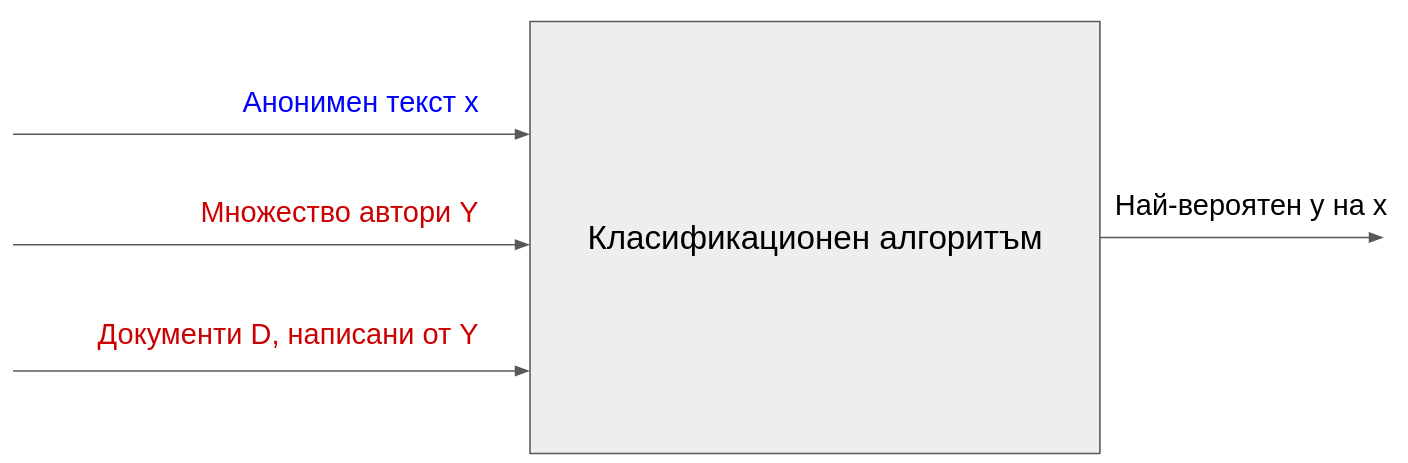
\includegraphics[scale=0.3]{./images/big_picture.png}
    \caption{Системата, представена "от птичи поглед".}
    \label{fig:bigP}
\end{figure}

\vspace{1em}

Обособени са пет модула, които формират процесите от свалянето на текстовете от Интернет пространството до изписване на информация за класификацията на даден текст в потребителския интерфейс. Те са:

\begin{enumerate}
    \item Модул scraper.py. Съдържа логиката за извличане на информация за текстовете от Интернет пространството и тяхното трансформиране в подходяща структура от данни, чрез която те да могат да бъдат обработени по лесен начин. Резултатът от използването на този модул е двумерна таблица, съставена от три колони: име на автор, име на произведение, път (т.е. URL) към Интернет ресурса, от които той може да бъде свален на локална машина.
    \item Модул downloader.py. Съдържа логиката за свалянето на текстовите ресурси от Интернет. Резултатът от използването на този модул е множество от текстови файлове, разположени в локални директория.
    \item Модул preprocessing.py. Съдържа логиката за обработка на текста преди подаването му към модел (т.е. класификатор). Резултатът от използването на този модул е списък от символни последователности (т.нар. "токени"). Реализацията предлага три нива на обработка, всяко от което добавя повече операции към (с други думи, надгражда) предишното. Те са уточнени в секция 4.1.
    \item Набор от Jupyter тетрадки. Съдържат логиката, която свързва гореизброените модули. Те предоставят възможност за изграждане на линейна и йерархична структура на кода. Използвани са за провеждането на експерименти и визуално проследяване на различните промени, които се правят върху двумерната таблица, използвана за създаване на тренировъчно, валидацинно, и тестово множество за класификационния модел.
    \item Модул app.py. Съдържа логиката за изграждането и обновяването на потребителския интерфейс, с който крайният потребител работи. Крайният резултат е интерактивен канал за комуникация с потребителя.
\end{enumerate}

\vspace{1em}
    
Изискванията за разработване на системата са:

\begin{enumerate}
    \item Създаване на паяк, копаещ документи (текстовете на съответните автори) от уеб страница.
    \item Създаване на модел, който е трениран върху тренировъчно множество ($80\%$ от данните), валидиран върху валидационно множество ($10\%$ от оставащи данни) и оценен върху тестово множество (последните $10\%$ оставащи данни).
    \item Сравняване на поне 3 стилистични метрики за всички автори.
    \item Сравняване на различни представяния на текст: \textit{tf-tdf} и \textit{transformer sentence embeddings}.
    \item Сравняване на класификатори: един и ансамбъл.
    \item Създаване на потребителски интерфейс.
\end{enumerate}

\vspace{1em}

Реализиран е и потребителски интерфейс, който е представен на .

    
%%%%%%%%%%%%%%%%%%%%%%%%%%%%%%%%%%%%%%%%%%%%%%%%%%
% Реализация, тестване/експерименти
%%%%%%%%%%%%%%%%%%%%%%%%%%%%%%%%%%%%%%%%%%%%%%%%%%

\section{Реализация, тестване/експерименти}

\subsection{Използвани технологии, платформи и библиотеки}

[ ] TODO: Подходящи средства за реализация за проекта (технологии, платформи и библиотеки). Избор на средствата и начин за използването им;

% describe the three levels for the tokenize functions.

\subsection{Реализация/Провеждане на експерименти}

[ ] TODO: Реализация (на модулите); 
За система/приложение: На кратко: планиране на тестването - тестови сценарии,...; Анализ на резултатите.


%%%%%%%%%%%%%%%%%%%%%%%%%%%%%%%%%%%%%%%%%%%%%%%%%%
% Заключение
%%%%%%%%%%%%%%%%%%%%%%%%%%%%%%%%%%%%%%%%%%%%%%%%%%

\section{Заключение}

[ ] TODO: Обобщение на направеното/резултатите. 
Идеи за по-нататъшно развитие, усъвършенстване или други експерименти.


%%%%%%%%%%%%%%%%%%%%%%%%%%%%%%%%%%%%%%%%%%%%%%%%%%
% Използвани технологии
%%%%%%%%%%%%%%%%%%%%%%%%%%%%%%%%%%%%%%%%%%%%%%%%%%

\section{Използвани технологии}

\begin{itemize}
    \item Python: програмен език, използван за създаването на Ati;
    \item Numpy: външна библиотека за бързи матрични и числови операции;
    \item Pandas: външна библиотека за манипулация на едномерни и двумерни данни;
    \item pickle: външна библиотека за запазване на структури във файловата система чрез създаване на бинарен .pkl файл;
    \item PyCaret: външна библиотека за автоматично създаване, трениране, валидиране и фино настройване на модели, основани на изкуствен интелект;
    \item Classla: външна библиотека за автоматично маркиране на частите на речта;
    \item selectolax: външна библиотека за извличане на информацията, съхранявана в HTML и CSS елементи, изграждащи и формиращи изгледа на уеб сайтове;
    \item bulstem: външна библиотека за връщане на думи към тяхната коренна форма;
    \item lemmagen3: външна библиотека за трансформиране на думи към техните т.нар "леми" - общи форми за голямо множество от думи;
    \item nltk: външна библиотека за обработка на естествен език;
    \item scikit-learn: външна библиотека за (ръчно) създаване, трениране, валидиране и фино настройване на модели, основани на изкуствен интелект;
    \item streamlit: външна библиотека за изграждане на уеб интерфейс.
\end{itemize}

\section{Използвана литература}

% Formatted using MLA style.
% статии, книги, онлайн ресурси

[1] Holmes, David I. “Authorship Attribution - Language Resources and Evaluation.” SpringerLink, Kluwer Academic Publishers, https://link.springer.com/article/10.1007/BF01830689. 

[2] Stamatatos, Efstathios. “Automatic Authorship Attribution.” ACM Digital Library, Association for Computational Linguistics, http://portal.acm.org/citation.cfm?doid=977035.977057. 

[3] Grieve, Jack. “Quantitative Authorship Attribution: An Evaluation of Techniques.” Digital Object Identifier System, Literary and Linguistic Computing, https://doi.org/10.1093/llc/fqm020. 

[4] Stamatatos, Efstathios. “A Survey of Modern Authorship Attribution Methods.” Wiley Online Library, Journal of the American Society for Information Science and Technology, https://onlinelibrary.wiley.com/doi/abs/10.1002/asi.21001. 

%%%%%%%%%%%%%%%%% END OF MAIN TEXT %%%%%%%%%%%%%%%%


\listoffigures

\end{document}